\begin{figure}[h!]
	\centering
	
	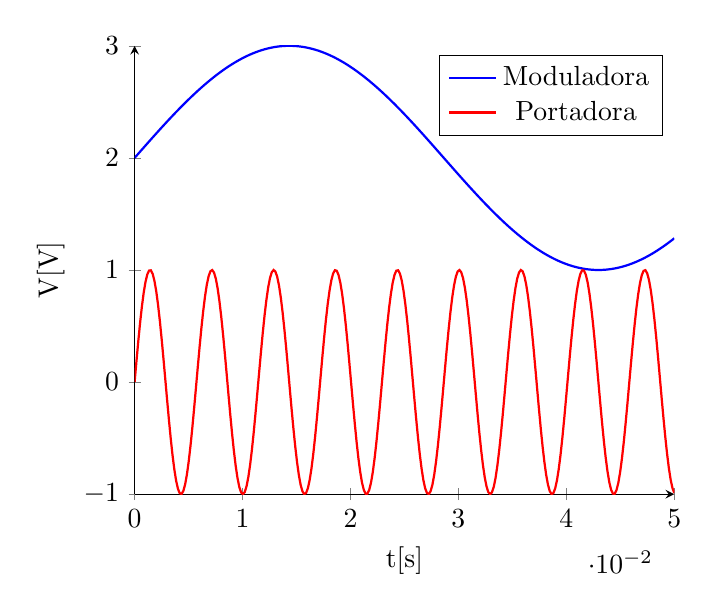
\begin{tikzpicture}
	\begin{axis}[
	axis lines = left,
	xlabel = {t[s]},
	ylabel = {V[V]},
	]
	
	%ENVOLVENTE SUPERIOR
	\addplot
	[thick=0.1cm,
	domain=0:0.05, 
	samples=300, 
	color=blue,
	]
	{sin(2*3.14159*x*1000)+2};
	
	
	
	\addplot
	[thick=0.1cm,
	domain=0:0.05, 
	samples=300, 
	color=red,
	]
	{sin(2*3.14159*x*10000)};
	
	%Se añade nota :D
	\addlegendentry{Moduladora}
	\addlegendentry{Portadora}
	
	\end{axis}
	\end{tikzpicture}
	\caption{Modulación AM}
	\label{modulacionAM}
\end{figure}